\documentclass[12pt,a4paper,bibliography=totocnumbered,listof=totocnumbered]{article}
\DeclareMathSizes{12}{12}{12}{12}
\usepackage[ngerman]{babel}
\usepackage[utf8]{inputenc}
\usepackage{amsmath}
\usepackage{amsfonts}
\usepackage{amssymb}
\usepackage{graphicx}
\usepackage{fancyhdr}
\usepackage{tabularx}
\usepackage{geometry}
\usepackage{setspace}
\usepackage[right]{eurosym}
\usepackage[printonlyused]{acronym}
\usepackage{subfig}
\usepackage{floatflt}
\usepackage[usenames,dvipsnames]{color}
\usepackage{colortbl}
\usepackage{paralist}
\usepackage{array}
%\usepackage{titlesec}
\usepackage{parskip}
\usepackage[right]{eurosym}
%\usepackage{picins}
\usepackage[subfigure,titles]{tocloft}
\usepackage[pdfpagelabels=true]{hyperref}
\usepackage{float}

\usepackage{listings}
\lstset{basicstyle=\footnotesize, captionpos=b, breaklines=true, showstringspaces=false, tabsize=2, frame=lines, numbers=left, numberstyle=\tiny, xleftmargin=2em, framexleftmargin=2em}
\makeatletter
\def\l@lstlisting#1#2{\@dottedtocline{1}{0em}{1em}{\hspace{1,5em} Lst. #1}{#2}}
\makeatother

\geometry{a4paper, top=27mm, left=20mm, right=20mm, bottom=35mm, headsep=10mm, footskip=12mm}


\hypersetup{unicode=false, pdftoolbar=true, pdfmenubar=true, pdffitwindow=false, pdfstartview={FitH},
	pdftitle={Wahlpflichtfach: Implementierung von Brettspielen am Beispiel ReversiXT (SS \the\year)},
	pdfauthor={Dr.\ Carsten Kern},
	pdfsubject={Projektbericht},
	pdfcreator={\LaTeX\ with package \flqq hyperref\frqq},
	pdfproducer={pdfTeX \the\pdftexversion.\pdftexrevision},
	pdfkeywords={Projektbericht, ReversiXT},
	pdfnewwindow=true,
	colorlinks=true,linkcolor=black,citecolor=black,filecolor=magenta,urlcolor=black}
\pdfinfo{/CreationDate (D:20151500000000)}
%\titlespacing{\section}{0pt}{12pt plus 4pt minus 2pt}{-6pt plus 2pt minus 2pt}

% Kopf- und Fusszeile
\renewcommand{\sectionmark}[1]{\markright{#1}}
\renewcommand{\leftmark}{\rightmark}
\pagestyle{fancy}
\lhead{}
\chead{}
\rhead{\thesection\space\contentsname}
\lfoot{Implementierung von Brettspielen am Beispiel ReversiXT -- SS \the\year}
\cfoot{}
\rfoot{\ \linebreak Seite \thepage}
\renewcommand{\headrulewidth}{0.4pt}
\renewcommand{\footrulewidth}{0.4pt}

% Vorspann
\renewcommand{\thesection}{\Roman{section}}
\renewcommand{\theHsection}{\Roman{section}}
\pagenumbering{Roman}

\newcommand{\folgen}[1]{
\ensuremath
#1
}

\newcommand{\MyTitlepage}[5][\empty]{
\thispagestyle{empty}
\begin{center}
	
\includegraphics[scale=0.2]{pics/oth-logo.png}\\
	\vspace*{2cm}
	\Large
	\textbf{Fakultät}\\
	\textbf{Informatik und Mathematik}\\
	\vspace*{2cm}
	\Huge
	\textbf{Projektbericht}\\
	\vspace*{0.5cm}
	\large
	zum Wahlpflichtfach im SS \the\year\\
	\vspace*{1cm}
	\textbf{Implementierung von Brettspielen am Beispiel ReversiXT}\\
	\vspace*{1cm}
	\includegraphics[height=6cm]{#1}
	\vfill
	\normalsize
	%\newcolumntype{x}[1]{>{\raggedleft\arraybackslash\hspace{0pt}}p{#1}}
	\begin{tabular}{rl}%{6cm}p{7.5cm}}
	    \rule{0mm}{5ex}\textbf{Gruppe:} & #2 \\
		\rule{0mm}{5ex}\textbf{Autoren:} & \hspace*{-0.5em}\begin{tabular}[t]{r}#3\end{tabular} \\ 
		\rule{0mm}{5ex}\textbf{Leiter:} & Prof. Dr. rer. nat. Carsten Kern \\ 
		\rule{0mm}{5ex}\textbf{Abgabedatum:} & #4 \\ 
	\end{tabular} 
\end{center}
\pagebreak
}

\begin{document}

% ----------------------------------------------------------------------------------------------------------
% Titelseite
% ----------------------------------------------------------------------------------------------------------
\MyTitlepage[pics/gruppenbild]{05}{
\texttt{robin.jahn@st.oth-regensburg.de}\\
\texttt{simon1.melcher@st.oth-regensburg.de}\\
\texttt{alexander1.wess@st.oth-regensburg.de}}
{27.06.\the\year}

\setcounter{page}{1} 
% ----------------------------------------------------------------------------------------------------------
% Inhaltsverzeichnis
% ----------------------------------------------------------------------------------------------------------
\tableofcontents
\pagebreak


% ----------------------------------------------------------------------------------------------------------
% Inhalt
% ----------------------------------------------------------------------------------------------------------
% Abstände Überschrift
%\titlespacing{\section}{0pt}{12pt plus 4pt minus 2pt}{6pt plus 2pt minus 2pt}
%\titlespacing{\subsection}{0pt}{12pt plus 4pt minus 2pt}{4pt plus 2pt minus 2pt}
%\titlespacing{\subsubsection}{0pt}{12pt plus 4pt minus 2pt}{2pt plus 2pt minus 2pt}

% Kopfzeile
\renewcommand{\sectionmark}[1]{\markright{#1}}
\renewcommand{\subsectionmark}[1]{}
\renewcommand{\subsubsectionmark}[1]{}
\lhead{Kapitel \thesection}
\rhead{\rightmark}

\onehalfspacing
\renewcommand{\thesection}{\arabic{section}}
\renewcommand{\theHsection}{\arabic{section}}
\setcounter{section}{0}
\pagenumbering{arabic}
\setcounter{page}{1}

% ----------------------------------------------------------------------------------
% Kapitel: Einleitung
% ----------------------------------------------------------------------------------
\section{Einleitung} \label{kap:Einleitung}
Der Begriff der \glqq künstlichen Intelligenz\grqq{} (kurz K.I.) ist heutzutage allgegenwärtig und findet in der Praxis immer mehr Anwendung und dementsprechend erhöht sich die Nachfrage an diesem Themengebiet.
%Quelle suchen?
Das Wahlpflichtfach \glqq ZOCK - Projekt Client-K.I.s für Brettspiele\grqq{} soll Studierenden einen ersten Einblick in die Algorithmen der künstlichen Intelligenz gewähren. Zur Umsetzung der Lernziele soll ein Projekt in Form einer Client-K.I. für das Spiel ReversiXT erstellt werden, wozu die Teilnehmer in Gruppen von je drei Studierenden aufgeteilt werden. 

Das Spiel ReversiXT basiert auf dem Brettspiel Reversi aus den 1880er Jahren und wurde um einige Sonderregelungen erweitert, um dessen Komplexität zu steigern damit umfassendere K.I.'s entwickelt werden können. Das Original wird von zwei Spielern auf einem acht mal acht Spielfeld gespielt, wie es in Abbildung \ref{fig:reversi_original_map} zu sehen ist, während es in der weiterentwickelten Version möglich ist, auf Karten mit bis zu 2500 Felder, also 50 mal 50, mit höchstens acht Spielern zu spielen. Ein Beispiel eines solchen Spielfelds wird in Abbildung \ref{fig:reversixt_circle_map} dargestellt. Hierbei handelt es sich um eine Karte für drei Spieler mit einer Höhe und Breite von je 29 Feldern, wobei auch verdeutlicht wird, dass Spielfelder nicht zwangsläufig quadratisch sein müssen, sondern individuell gestaltet werden können.

\vspace{1em}
\begin{minipage}{\linewidth}
	\centering
	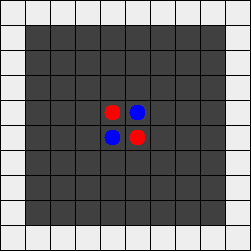
\includegraphics[width=0.4\linewidth]{pics/reversi_original_map.png}
	\captionof{figure}[Bsp. 1 Reversi Karte]{Originales Spielfeld Reversi}
	\label{fig:reversi_original_map}
\end{minipage}
\\

\vspace{1em}
\begin{minipage}{\linewidth}
	\centering
	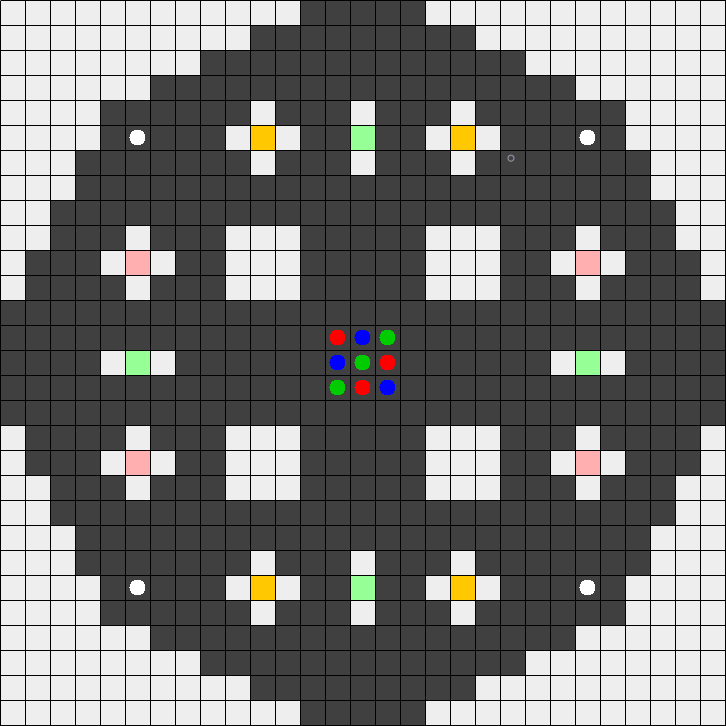
\includegraphics[width=0.7\linewidth]{pics/reversixt_circle_map.png}
	\captionof{figure}[Bsp. 2 ReversiXT Circle Karte]{Spielfeld ReversiXT}
	\label{fig:reversixt_circle_map}
\end{minipage}
\\

Jedem Spieler wird zu Beginn eine Farbe und die dazugehörigen Spielsteine zugewiesen. Das Spielprinzip ist es dann von den eigenen Steinen aus über die der Gegner auf ein freies Feld zu legen, wodurch die eingeschlossenen gegnerischen Steine eingefärbt werden und den Besitzer wechseln. Das bedeutet, dass zwischen dem eigenen Stein und dem freien Feld immer mindestens ein gegnerischer liegen muss. Es kann generell in jede Richtung, horizontal, vertikal und diagonal gezogen werden. Ein Beispiel hierfür ist in den folgenden Abbildungen zu sehen wobei Abbildung \ref{fig:capture_pre} die Situation vor dem Zug des Spielers mit den roten Steinen zeigt und durch eine weiße Umrandung verdeutlicht werden soll auf welches Feld gezogen wird. Abbildung \ref{fig:capture_post} stellt den Spielfeldzustand nach des Färbens dar.

\begin{figure}[H]
\centering
\begin{minipage}[c]{0.4\textwidth}
	\centering
	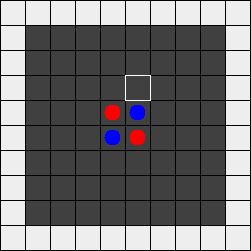
\includegraphics[width=\textwidth]{pics/reversi_original_map_capture_1.png}
	\captionof{figure}[Bsp. 3 Einfärbern vorher]{Einfärben vor dem Zug}
	\label{fig:capture_pre}
\end{minipage}
\hspace{0.1\textwidth}
\begin{minipage}[c]{0.4\textwidth}
	\centering
	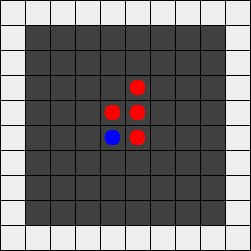
\includegraphics[width=\textwidth]{pics/reversi_original_map_capture_2.png}
	\captionof{figure}[Bsp. 4 Einfärbern nachher]{Einfärben nach dem Zug}
	\label{fig:capture_post}
\end{minipage}
\end{figure}

Die erweiterte Variante bietet eine weitere Besonderheit bei der Möglichkeit einen gültigen Zug durchzuführen in Form von sogenannten Überschreibsteine. Diese erlauben es nicht nur auf freie Felder zu legen, sondern auch auf eigene oder gegnerische Steine, um diese einzunehmen, sofern es sich um einen ansonsten regelkonformen Spielzug handelt. Wie viele dieser Steine jeder Spieler zu Beginn zur Verfügung hat, wird vom Ersteller der Karte vorgeschrieben. Es ist jedoch möglich (abhängig vom Spielfeld) zusätzliche dieser Steine im Laufe der Runde zu erhalten, worauf im Weiteren noch genauer eingegangen wird. 
%Bsp. Überschreibsteine

Außerdem können ReversiXT Karten besondere Felder enthalten, die ausgelöst werden sobald ein Spieler das erste Mal darauf zieht. Dazu gehören die Bonusfelder, die dem Spieler die Wahl zwischen einer zusätzlichen Bombe oder eines Überschreibsteins gibt (In Abbildung \ref{fig:reversixt_circle_map} in gelb dargestellt). Setzt ein Spieler auf ein Inversionsfeld werden die Farben der Spieler um eins verschoben, wodurch bspw. Spieler 2 die Steine von Spieler 1, Spieler 3 die von Spieler 2 und Spieler 1 die von Spieler 3 erhält (in Abbildung \ref{fig:reversixt_circle_map} in rosa). Ein Wahlfeld gibt einem Spieler die Möglichkeit seine Steine gezielt mit denen eines Gegners zu tauschen, allerdings kann auch darauf verzichtet werden indem mit den eigenen Steinen \glqq getauscht\grqq{} wird (In Abbildung \ref{fig:reversixt_circle_map} in grün). Als letzte Art von Sonderfeldern sind die Expansionsfelder zu nennen, die für alle Spieler als Gegner gelten. Eine weitere Besonderheit dieser Felder ist, dass sie zu jeder Zeit mit einem Überschreibstein eingenommen werden können, selbst wenn dadurch kein gültiger Zug entsteht (In Abbildung \ref{fig:reversixt_circle_map} als weiße Spieler dargestellt). Durch diese Steine können einige interessante Spielfelder entstehen. Es können zum Beispiel Spielfelder gebaut werden, bei denen die Spieler zu Beginn keine eigenen Steine besitzen, es jedoch einige Expansionsfelder gibt. In diesem Fall könnten sich die Spieler in den ersten Zügen aussuchen, auf welchen Expansionsstein sie Ziehen möchten. Dieser Ansatz wurde bei der Karte in Abbildung \ref{fig:reversixt_circle_map} verfolgt. Eine weitere Konsequenz von Expansionsfeldern ist, dass abgeschnittene Bereiche einer Karte bespielbar werden, solange dort einige Expansionssteine platziert wurden.

Eine andere Eigenart von ReversiXT sind die Transitionen, die wie eine Art Portal betrachtet werden können. Sie erlauben es über die Wände der Karte hinaus zu ziehen, um an einer andere Stelle der Karte (das andere Ende der Transition) herauszukommen. Diese sind ebenfalls optional und können vom Ersteller des jeweiligen Spielfelds gezielt gesetzt werden. Dadurch können Karten bspw. in einzelne Bereiche eingeteilt werden, die nur über Transitionen erreicht werden können, wie es in Abbildung \ref{fig:reversixt_islands_map} dargestellt wird. Die Transitionen werden hierbei durch gelbe Linien repräsentiert und bestehen aus einem Ein- und Ausgangsfeld sowie einer Richtung in die diese Transition gültig ist. Ebenso ist zu beachten, dass diese immer in beide Richtungen genutzt werden können.
%Beispiel Zug mit Transition?
%Loops

\vspace{1em}
\begin{minipage}{\linewidth}
	\centering
	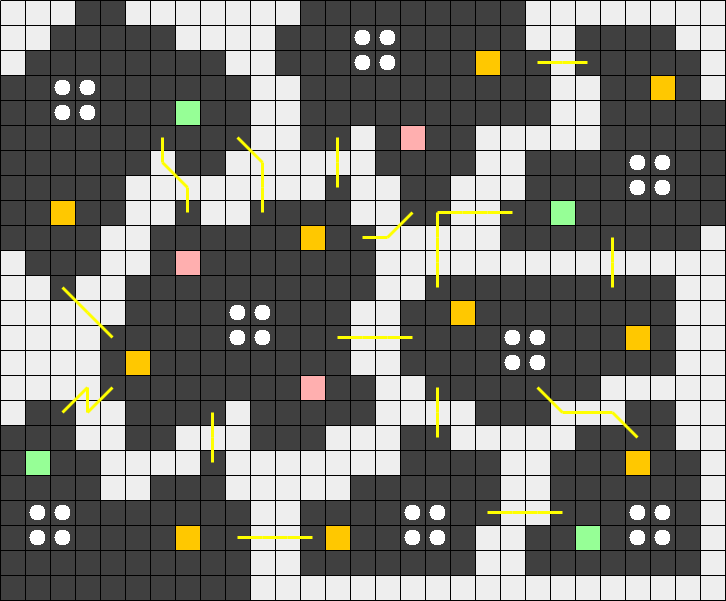
\includegraphics[width=0.7\linewidth]{pics/reversixt_islands_map.png}
	\captionof{figure}[Bsp. 3 ReversiXT Islands Karte]{Spielfeld mit Transitionen}
	\label{fig:reversixt_islands_map}
\end{minipage}
\\

Aufgrund dieser Besonderheit ist es möglich in Schleifen über die Karte zu gehen, weshalb besonders bei der Durchführung von Zügen darauf geachtet werden muss, dass keine ungültigen Züge getätigt werden. Abbildung \ref{fig:example_transition_loop} zeigt eine solche Situation beispielhaft. Sollte ein Spieler auf das dort dargestellte Expansionsfeld mit einem Überschreibstein ziehen, dürfen die blauen Steine nicht eingefärbt werden, da er sie zwar über die Transition einschließt, dies jedoch mit ein und demselben Stein macht, was gegen die Regeln verstoßt.

\vspace{1em}
\begin{minipage}{\linewidth}
	\centering
	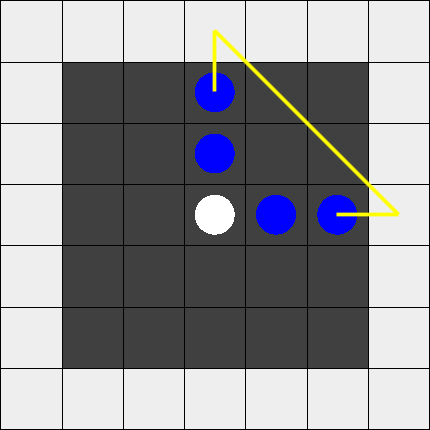
\includegraphics[width=0.4\linewidth]{pics/transition_loop.png}
	\captionof{figure}[Bsp. 4 Transition loop]{Transition mit Schleife}
	\label{fig:example_transition_loop}
\end{minipage}
\\

Das Spiel endet sobald kein Spieler mehr einen gültigen Zug machen kann. In der herkömmlichen Version wird an dieser Stelle der Gewinner ermittelt, indem die Anzahl der Steine der Spieler in deren Farbe verglichen wird und derjenige gewinnt, der die meisten einfärben konnte. ReversiXT erweitert das Spielprinzip um eine weiter Spielphase, in der Bomben geworfen werden können. Die Anzahl wie viele Bomben jeder Spieler initial besitzt sowie deren Stärke wird zu Beginn der Partie festgelegt und kann je nach Spielfeld variieren. Bomben der Stärke zwei zerstören bspw. das Feld an dem sie platziert werden sowie alle Felder, die innerhalb von zwei Schritten vom Zentrum aus erreichbar sind, wobei auch über Transitionen hinweg gegangen werden kann, wodurch diese ebenfalls entfernt werden. Deshalb können Bomben eine wertvolle Ressource darstellen, da sie gezielt auf die gegnerischen Steine eingesetzt werden können. Nach dieser Phase wird der Sieger wie im klassischen Reversi bestimmt.


\newpage
% ----------------------------------------------------------------------------------
% Kapitel: Allgemeine Informationen
% ----------------------------------------------------------------------------------
\section{Allgemeine Informationen}
Wie in Kapitel \ref{kap:Einleitung} erwähnt wurde das Projekt in einer Kleingruppe von drei Studierenden durchgeführt, weshalb in diesem Kapitel darauf eingegangen wird, wer Teil der Gruppe 05 war, welche Vorkenntnisse vorhanden waren, wie kommuniziert wurde sowie welche technische Mittel verwendet wurden (Soft- und Hardware). Dies soll einen Einblick gewähren, auf welcher Basis das Projekt umgesetzt wurde.

\subsection{Team und Kommunikation}
Die Mitglieder der Gruppe 05 waren Simon Melcher, Robin Jahn und Alexander Wess, die sich alle im vierten Semester ihres Bachelor Informatik Studiums befanden.

Wichtiges Vorwissen wurde vor allem aus den Fächern Programmieren 2 und Algorithmen und Datenstrukturen von den Studierenden mitgebracht. Dort wurde u. a. anhand von Java die Objektorientierte Programmierung vermittelt, anhand dieser dann verschiedenste Algorithmen in anderen Modulen besprochen und eigene Projekte durchgeführt wurden. Außerdem wurde ein Grundverständnis von Komplexität von Algorithmen mitgebracht, wodurch stärker auf Performance geachtet werden konnte und Einschätzungen getroffen werden konnten, welche Datenstruktur an welcher Stelle sinnvoll war. Robin Jahn konnte sich bereits im Vorfeld wissen zu verschiedenen K.\,I.\ relevanten Themen durch den Austausch mit anderen Studierenden des Studiengangs \glqq Künstliche Intelligenz und Data Science \grqq{} an der OTH Regensburg aneignen.

Neben der wöchentlichen Vorlesung und Übung der Veranstaltung, wurde jeden Freitag eine Besprechung mit allen Mitgliedern abgehalten. In diesen Besprechungen wurden die Aufgaben, die bereits in der Übung am Dienstag verteilt wurden, besprochen und aufgetretene Probleme gemeinsam gelöst. Außerdem wurden neue Ansätze zur Ausarbeitung bzw. Verbesserung des Clients diskutiert und implementiert sowie neue Aufgaben zur Bearbeitung über das Wochenende zugeteilt. Zusätzlich wurde über eine gemeinsame WhatsApp Gruppe kommuniziert, in der Fragen gestellt werden konnten und organisatorisches vereinbart wurde.

\vspace{1em}
\begin{table}[H]
\centering
	\begin{tabular} {| m{2.6cm} | m{4cm} | m{4cm} | m{4cm}|}
		\hline
		\textbf{} &\textbf{Simon Melcher} & \textbf{Robin Jahn} & \textbf{Alexander Wess}\\
		\hline
		Woche 1 & Erstellen von eigenen Spielfeldern & Erstellen von eigenen Spielfeldern; Implementierung der Datenstruktur, Einlesen und Ausgabe & Erstellen von eigenen Spielfeldern\\
		\hline
		Woche 2 & Programmierung der gültigen Züge für Spezialfelder & Programmierung der gültigen Züge & Beschreibung der Zugheuristiken im Projektbericht\\
		\hline
		Woche 3 & Umsetzung der verbesserter Heuristik & Umsetzung der verbesserter Heuristik & Projektbericht Kapitel 1 - 3\\
		\hline
		Woche 4 & \textit{Krank} & Programmierung der Netzwerkfunktionalität & Erstellung des Build-File\\
		\hline
		Woche 5 & Implementierung Client-Parameter & Implementierung Paranoidsuche &\\
		\hline
		Woche 6 & Skripte erstellt um Tests durchzuführen & Skripte erstellt um Tests durchzuführen; Statistik implementiert; Bombenphase programmiert & Implementierung Alpha-Beta-Pruning\\
		\hline
		Woche 7 & Implementierung Iterative-Deepening & Implementierung Zugsortierung & Erweiterung des Projektberichts\\
		\hline
		Woche 8 & Programmierung einer neuer Funktion für die Bombenphase zum zählen der Steine & Änderung des Skripts zur Ermittlung der besten Multiplikatoren für die Heuristik & Implementierung einer neuen Funktion zur Bewertung von Bonusfeldern\\
		\hline
		Woche 9 & Implementierung Killer Heuristik und BRS+ & Programmierung einer neuen Funktion zur Zugermittlung & Implementierung BRS+; Weiterführung des Projektberichts\\
		\hline
		Woche 10 & Implementierung Zobrist Hasing und Aspiration Window & Implementierung MCTS & Implementierung Methode zufälliger Zug\\
		\hline
		Woche 11 - 13 & Optimierungen & Optimierungen & Optimierungen\\
		\hline
	\end{tabular}
	\caption{Aufgabenverteilung}
	\label{tab:tasks}
\end{table}

\subsection{Technische Daten}
In diesem Abschnitt soll auf die verwendeten technischen Mittel eingegangen werden. Das Projekt wurde in der Programmiersprache Java in der 11ten Version umgesetzt, da zum einen in dieser Programmiersprache bereits die meiste Erfahrung gesammelt werden konnte. Zum anderen konnten die gängigen Vorteile dieser Programmiersprache genutzt werden, wie z. B. die automatische Speicher- und Heap-Verwaltung oder die Möglichkeit mit \glqq Call by Reference\grqq{} zu arbeiten ohne Pointer zu benutzen.
Zu Beginn legte sich die Gruppe fest einheitlich die Entwicklungsumgebung IntelliJ IDEA der Version 2021.3.3 von JetBrains zu nutzen. Der Vorteil davon war u. a., dass diese bereits eine gute Anbindung an Git besitzte und somit das Arbeiten in einem gemeinsam Repository signifikant erleichterte.
Als Betriebssystem wurde hauptsächlich Windows 10 der Version 21H2 verwendet. Außerdem wurde von Robin Jahn eine virtuelle Maschine (VM) eingerichtet, die das Unix Betriebssystem Ubuntu simulierte. Simon Melcher und Alexander Wess nutzten hingegen das Windows Subsystem for Linux (WSL). Einerseits konnte mittels Linux der Server ausgeführt werden, wodurch neuer Code direkt im Spiel ausprobiert werden konnte. Außerdem konnten durch die Verwendung von WLS und der VM unterschiedliche Probleme identifiziert werden, die spezifisch auf einer der Umgebungen aufgetreten sind. Dadurch sollte sichergestellt werden, dass der entwickelte Client fehlerlos über ein Linux Betriebssystem ausgeführt werden konnte und die Kommunikation mit dem Server reibungslos funktionierte.

Ebenfalls wurden die Tools aus dem globalen Repository wie der Map Editor genutzt, um Spielfelder zu erstellen und zu bearbeiten. Zusätzlich wurden Skripte angefertigt, die die Erstellung des Projekts erleichtern sollten. Um den Server auf dem die Spiele ausgetragen wurden und die zur Verfügung gestellte triviale K.I., nicht nach jedem Spiel neu starten zu müssen, wurde ein Skript programmiert, das nach jeder Partie dies übernahm. Zur Verbesserung der Heuristik, die in Kapitel \ref{kap:Heuristik_Beschreibung} genauer beschrieben wird, wurde ein Skript entwickelt, das verschiedene Möglichkeiten zur Gewichtung der Bewertungsfunktionen automatisch testete und die beste Kombination zurückgab.

Robin Jahn entwickelte zu Beginn auf seinem Laptop mit einem AMD Ryzen 5 3500U Prozessor, der eine Taktfrequenz von 2,1 bis 3,7 GHz aufweist, und 8 GB Arbeitsspeicher. Jedoch wechselte er, vor allem zum Testen, auf seinen Tower PC, der mit einem Intel Core i5-7600 (3,5 GHz), 16GB RAM und einer Nvidia GeForce GTX 1070 Grafikkarte ausgestattet war, da dieser die virtuelle Maschine aufgrund seiner höheren Leistung besser bewältigen konnte. Simon Melcher wechselte ebenfalls zwischen einem Desktop Computer und einem Laptop für die Vorlesungen, Übungen und Gruppenmeetings. Beide Geräte besaßen 16 GB RAM sowie einen AMD Ryzen 5 2600X (3,6 GHz), der in seinem PC enthalten war und einen AMD Ryzen 3500U (2,1 GHz) in seinem Laptop. Alexander Wess arbeitet durchgehend mit einem Laptop, der einen AMD Ryzen 5 5500U (2.10 GHz) Prozessor und 16 GB Arbeitsspeicher verbaut hatte.

\newpage
% ----------------------------------------------------------------------------------
% Kapitel: Spielfeldbewertung
% ----------------------------------------------------------------------------------
\section{Spielfeldbewertung}
Zur Umsetzung eines solchen Clients wird eine K.I. benötigt, die anhand von Suchbäumen entscheidet, welcher Zug als nächstes getätigt werden soll. Die Elemente dieses Suchbaums sind verschiedene Szenarien, die aus der aktuellen Situation auf dem Spielfeld entstehen können. Hierfür müssen die verschiedenen Zugmöglichkeiten simuliert und der daraus entstandene Zustand bewertet werden, um zu entscheiden welcher der bestmögliche Zug ist. 
In diesem Kapitel soll deshalb darauf eingegangen werden, wie Gruppe fünf diese Einschätzung umgesetzt hat.

\subsection{Bestandteile}\label{kap:Heuristik_Beschreibung}
Eine mögliche Heuristik zur Spielfeldbewertung ist die eigene Flexibilität in Bezug auf durchführ"-bare Spielzüge (in diesem Kontext auch als "Mobilität" bezeichnet), die sich aus der jeweiligen Situation ergeben. Hierbei ist der Grundgedanke der, dass der Spieler nicht nur darauf achtet möglichst viele Steine auf dem Feld zu haben bzw. beim Tätigen eines Spielzugs möglichst viele Steine einzufärben (Greedy-Verfahren), sondern ebenfalls zu berücksichtigen wie viele Optionen er hat das Spiel weiterzuführen. Mehr valide Züge als die Gegner zu haben ist dementsprechend von Vorteil. Dadurch soll sichergestellt werden, dass die eigene Strategie weiterverfolgt werden kann und nicht der Gegner den Spielverlauf vorgibt oder man zu \glqq schlechten\grqq{} Zügen gezwungen wird.

Die zuvor beschriebene Situation ist in Abbildung \ref{fig:example_heuristics_flexibility_simple} zu sehen. Der Spieler mit den blauen Steinen hat zwar mehr eingefärbt, kann jedoch nicht mehr ziehen (sofern keine Überschreibsteine verfügbar sind) und muss abwarten, was der Spieler mit den roten Steinen als nächstes macht. Dieser kann hingegen frei entscheiden in welche Richtung die Karte als nächstes bespielt werden soll, da er mehrere Richtung ziehen kann.

Jedoch bringt dieses Verfahren auch Nachteile mit sich, da das Ziel des Spiels, am Ende der Partie die meisten Steine auf dem Spielfeld zu haben, vernachlässigt wird.

\vspace{1em}
\begin{minipage}{\linewidth}
	\centering
	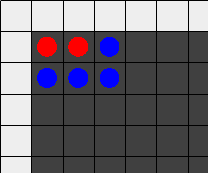
\includegraphics[width=0.3\linewidth]{pics/heuristics_flexibility_simple_v2.png}
	\captionof{figure}[Bsp. 1 Heuristik Flexibilität]{Situation Blau kann nicht mehr ziehen}
	\label{fig:example_heuristics_flexibility_simple}
\end{minipage}
\\


Zur Umsetzung der Spielfeldbewertung hinsichtlich der Anzahl an Steinen und der Mobilität wurde das gleiche Vorgehen verwendet. Im Folgenden wird die Umsetzung für die Anzahl der Steine beschrieben.
Zuerst wird die Anzahl der eigenen Steine und die Anzahl der gefärbten Steine bestimmt. Durch den Quotient dieser beiden Werte bekommt man den Anteil der eigenen Steine zu allen Steinen, die bisher eingenommen wurden. Wenn man z.B. 25 von insgesamt 100 gefärbten Steinen besitzt hat man 25\% der Steine. Dieser Anteilswert hat jedoch je nach Anzahl der Spieler auf einer Karte eine andere Aussagekraft. Wenn man 25\% der Steine auf einer 2-Spieler Karte hat ist dieser Wert ziemlich schlecht. Wenn es jedoch eine 4 Spieler Karte ist, ist es der durchschnitt. Um dieses Problem zu lösen wird der Wert noch normiert, indem er durch die Durchschnittsanzahl der Steine pro Spieler geteilt wird. 

Insgesamt ergibt sich
\( \frac{ \frac{\text{ \# meine Steine}}{\text{ \# gefärbte Steine}} }{ \frac{1}{ \# Spieler} } \).
Was zu
\( \frac{ \text{ \# meine Steine } \cdot \text{ \# Spieler} }{ \text{ \# gefärbte Steine} } \) 
vereinfacht werden kann.\\
Wenn das Endergebnis 1 ist bedeutet dies, dass der Spieler genau so viele Steine besitzt, wie er im durchschnitt besitzen sollte. Ist es 0.5 oder auch 50\% hat der Spieler nur 50\% der Steine die er im durchschnitt besitzen sollte. Ebenso hat er beim Wert 1,5 150\% der durchschnittlichen Steine.
Im Vergleich zu einem Absolutwert hat diese Methode einige Vorteile. Da die Werte unabhängig von der Anzahl der Spieler oder des Spielfortschritts sind  kann ein Multiplikator auf den Wert gerechnet werden um das Gewicht dieser Bewertungsmethode gegenüber den anderen zu verändern. Dieses ist durch die Unabhängigkeit auf allen möglichen Karten gleich, was dem gewünschten Verhalten entspricht.

Wie schon oben erwähnt kann das gleiche Verfahren auch für die Bewertung der Mobilität verwendet werden. In diesem Fall sieht die Formel wie folgt aus:
\[ \frac{ \text{ \# meine Züge } \cdot \text{ \# Spieler } }{ \sum_{i=1}^{ \#Spieler} \text{ \# züge von Spieler i } }  \].


Ein weiterer Ansatz der Spielfeldbewertung ist die \glqq Sicherheit\grqq{} der einnehmbaren Felder. In diesem Fall soll darauf geachtete werden, ob und wie leicht die jeweiligen Felder vom Gegner eingefärbt werden können. Folglich muss hierbei überprüft werden, ob ein Feld, nachdem es das erste Mal besetzt wird, überhaupt noch einmal den Besitzer wechseln kann oder aus wie vielen Richtungen die Gegner noch Möglichkeiten haben, dieses Feld zurückzugewinnen. Zusätzlich soll einkalkuliert werden, wie viel Prozent der bespielbaren Felder ausgehend von dieser Position erreichbar sind. Diese Analyse wird anhand eines Punktesystems realisiert, auf das im weiteren Verlauf dieses Kapitels noch genauer eingegangen wird.

Das naheliegendste Beispiel für ein solches sicheres Feld ist eine Ecke wie in Abbildung \ref{fig:example_heuristics_safe_fields_corner} dargestellt. Dieser Stein kann weder horizontal noch vertikal oder diagonal von einem Gegner eingefärbt werden und stellt somit eine wertvolle Position dar. Aufgrund der zusätzlichen Regeln von ReversiXT können diese Felder zwar noch mit Überschreibsteine eingenommen werden, jedoch muss dafür eine begrenzte und wertvolle Ressource verwendet werden.

\vspace{1em}
\begin{minipage}{\linewidth}
	\centering
	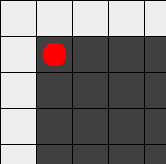
\includegraphics[width=0.3\linewidth]{pics/heuristics_safe_fields_corner.png}
	\captionof{figure}[Bsp. 1 Heuristik sichere Felder]{Nicht einnehmbares Feld mit vielen 		Zugmöglichkeiten}
	\label{fig:example_heuristics_safe_fields_corner}
\end{minipage}
\\

Abbildung \ref{fig:example_heuristics_safe_fields_dead_end} zeigt eine andere Situation, in der das Feld zwar ebenfalls nicht mehr mit einem herkömmlichen Zug eingenommen werden kann, jedoch auch nur eine Richtung (nach Unten) als Zugmöglichkeit bietet. Somit kann von hieraus nur ein geringer Prozentsatz der Karte bespielt werden und sollte schlechter eingestuft werden als das Feld aus der Situation davor.

\vspace{1em}
\begin{minipage}{\linewidth}
	\centering
	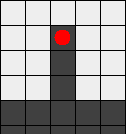
\includegraphics[width=0.3\linewidth]{pics/heuristics_safe_fields_dead_end.png}
	\captionof{figure}[Bsp. 2 Heuristik sichere Felder]{Nicht einnehmbares Feld mit wenigen Zugmöglichkeiten}
	\label{fig:example_heuristics_safe_fields_dead_end}
\end{minipage}
\\

Ein Feld, das sich am Rand der Karte befindet, kann zwar eingenommen werden, jedoch sind die Möglichkeiten beschränkt, da es lediglich vertikal von gegnerischen Spielern eingefärbt werden kann, wie es in Abbildung \ref{fig:example_heuristics_safe_fields_outer_side} zu sehen ist. Gleichzeitig eröffnet es Möglichkeiten in fünf Richtungen den nächsten Spielzug durchzuführen.

%ToDo: Pfeile einfügen
\vspace{1em}
\begin{minipage}{\linewidth}
	\centering
	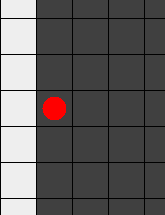
\includegraphics[width=0.3\linewidth]{pics/heuristics_safe_fields_outer_side.png}
	\captionof{figure}[Bsp. 3 Heuristik sichere Felder]{Beschränkt einnehmbares Feld}
	\label{fig:example_heuristics_safe_fields_outer_side}
\end{minipage}
\\

Wenn jedoch keine Seite durch das Ende der Karte geschützt ist, ist dieses Feld von allen Seiten für den Gegner erreichbar, bietet jedoch gleichzeitig viele Zugmöglichkeiten. Deshalb muss es durchdacht werden, wann welche Position wichtiger ist. In Abbildung \ref{fig:example_heuristics_safe_fields_middle} wird dies durch ein Feld inmitten der Spielfläche verdeutlicht.

%ToDo: Pfeile einfügen
\vspace{1em}
\begin{minipage}{\linewidth}
	\centering
	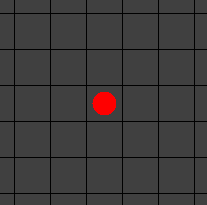
\includegraphics[width=0.3\linewidth]{pics/heuristics_safe_fields_middle.png}
	\captionof{figure}[Bsp. 4 Heuristik sichere Felder]{Voll einnehmbares Feld}
	\label{fig:example_heuristics_safe_fields_middle}
\end{minipage}
\\

Die Schwierigkeit dieser Heuristik besteht darin, dass die Sonderregeln von ReversiXT nicht vernachlässigt werden dürfen. Ein vermeintlich sicheres Feld (z. B. eine Ecke), kann durch Transitionen gar kein uneinnehmbares Feld sein und muss auch als dieses behandelt werden. Ebenso können Überschreibsteine diesen Effekt hervorrufen.

Wie bereits zuvor erwähnt wurde die Analyse zur Sicherheit der Felder bzw. deren Wert anhand eines Punktesystems realisiert. Hierbei wurde jedem Feld eine Zahl zugeordnet, die auf Basis von einigen Kriterien errechnet wurde und somit darstellte, wie bedeutend dieses ist. Zuvor wurde bereits erläutert, dass zum einen die Möglichkeiten der Gegner zur Eroberung des Feldes als auch die daraus ausgehenden Wege maßgebend sind. Zusätzlich wurde berücksichtigt wie weit von den jeweiligen Positionen aus gezogen werden kann bzw. wie viel Prozent des Spielfelds davon ausgehend erreichbar ist. Dadurch sollte sichergestellt werden, dass z.B. Felder, die zwar nicht mehr eingenommen werden können, aber sich bspw. in schmäleren Bereichen der Karte befinden und somit weniger Zugmöglichkeiten bieten, nicht so gut bewertet werden, wie welche von denen aus weit ins Spielfeld hinein gezogen werden kann. Der Stein, der in Abbildung \ref{fig:example_heuristics_reachable_fields} zu sehen ist, ist ein Beispiel für ein solches Feld. Ein gegnerischer Spieler kann diesen Stein zwar nicht mehr erobern, aber gezogen werden kann von hier aus nur nach oben, da links und diagonal nur ein Feld bis zum Ende der Karte ist.

\vspace{1em}
\begin{minipage}{\linewidth}
	\centering
	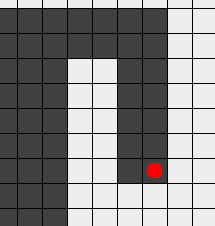
\includegraphics[width=0.5\linewidth]{pics/heuristics_reachable_fields.png}
	\captionof{figure}[Bsp. 1 Heuristik erreichbare Felder]{Feld mit beschränkten Zugmöglichkeiten}
	\label{fig:example_heuristics_reachable_fields}
\end{minipage}
\\

%Bonusfeldbewertung
Ebenso wurden die speziellen Felder von ReversiXT höher eingestuft als normale, sodass bspw. ein Bonusfeld immer eingenommen wird, sofern es möglich ist. 
%Waves
Um sicher zu gehen, dass der eigene Client vorteilhafte Felder auch einnehmen kann wurde ein Algorithmus entworfen, der die angrenzenden Bereiche mit negativen Zahlen gewichtet. Dadurch sollte signalisiert werden, dass diese Felder gemieden werden sollten, da sie dem Spieler die Chance verwehen auf eines der positiven Felder zu ziehen und nur dem Gegner die Gelegenheit dafür geben würde. Hierbei wurde jedoch darauf geachtet, dass vorteilhafte Felder sich nicht gegenseitig beeinflussen, da z. B. mehrere Bonusfelder, die direkt nebeneinander liegen ansonsten die Bewertung verfälscht hätten und möglicherweise sogar geringer eingestuft werden würden als gewöhnliche. Gebiete, die wiederum an solche negativ eingeschätzten Felder angrenzen wurden wieder positiv beziffert, womit das Ziel verfolgt wurde, dass der eigene Client auf diese zieht, um den Gegner dazu zu bringen, dass er auf ein Feld, das sich um ein nutzbringendes Feld befindet zu legen. Dieses Verfahren von abwechselnder negativen und positiven Bewertung ausgehend von dem bedeutenden Feld, wurde weitergeführt, wodurch eine Art Wellen entstanden.
Im Laufe der Entwicklung zeigte sich, dass eine statische Berechnung dieser Wellen nicht gewinnbringend war, da Felder, wie bspw. Bonusfelder weiterhin positiv dargestellt wurden selbst, wenn diese bereits von einem Gegner eingenommen wurden und somit keinen zusätzliche Ressource mehr brachten. Dadurch bevorzugte der Client weiterhin diese Spielfelder z. B. beim durchführen von Überschreibzügen, obwohl es sich lediglich um ein normales Feld handelte.

Abschließend wurden die Werte der einzelnen Heuristikbestandteile addiert. Das Endergebnis einer solchen Berechnung ist in Abbildung \ref{fig:example_heuristics_implementation_field_values_matrix} zu sehen. Hier ist deutlich zu erkennen, dass Felder in den Ecken oder am Rand höher beziffert wurden als welche in der Mitte der Karte.
%neues Bild

\vspace{1em}
\begin{minipage}{\linewidth}
	\centering
	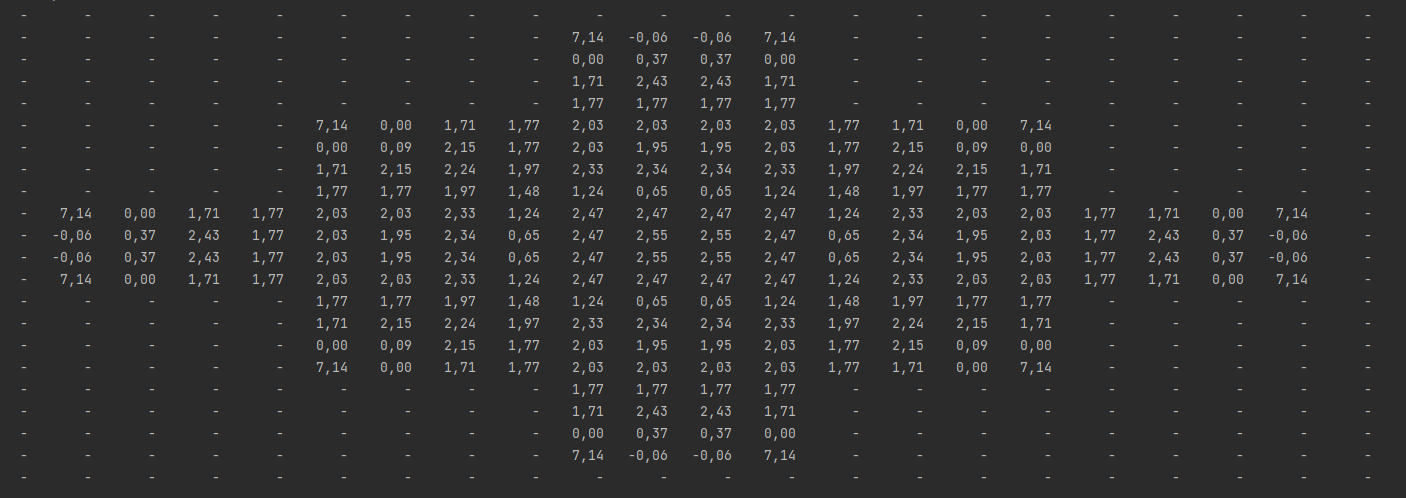
\includegraphics[width=0.8\linewidth]{pics/heuristics_implementation_field_values_matrix.png}
	\captionof{figure}[Bsp. 1 Heuristik Implementierung Bewertung Felder]{Spielfeld mit Punktzahl zur Bewertung der Felder}
	\label{fig:example_heuristics_implementation_field_values_matrix}
\end{minipage} 
\\

Die einzelnen Komponenten der Heuristik wurden mithilfe von Multiplikatoren verschieden stark priorisiert. Während der Entwicklung des Clients wurde ersichtlich, dass die unterschiedlichen Bewertungsmethoden im Laufe eines Spiels unterschiedlich schwer gewichtet werden sollten. Deshalb wurde ein Algorithmus entworfen, der angibt wie viele Felder auf einer Karte tatsächlich bespielbar sind. Woraufhin verschiedene Phasen implementiert wurden, die angaben wie weit das Spiel bereits vorangeschritten ist und die Multiplikatoren der einzelnen Heuristiken wurden abhängig davon neu gesetzt. In der ersten Phase befand sich die Partie solange weniger als 50\% der bespielbaren Felder eingenommen wurden. Verschiedene Tests zum finden der optimalen Multiplikatoren ergaben, dass zu diesem Zeitpunkt vor allem wichtig war wie weit von diesem Feld gezogen werden kann. War der Wert der eingefärbten Felder zwischen 50\% und 80\% befand sich das Spiel in der Mitte und somit in Phase 2. Hier wurde noch zusätzlich der Multiplikator für die Anzahl der einzufärbenden Steine deutlich erhöht während die anderen kaum verändert wurden. Ab 80\% Füllmenge des Spielbretts wurden die Multiplikatoren für Phase 3 gesetzt, in der die Mobilität an Wichtigkeit zunahm.
 
\newpage
% ----------------------------------------------------------------------------------
% Kapitel: Zusätzliche Inhalte
% ----------------------------------------------------------------------------------
\section{Optimierungen}
\subsection{Aspiration Window}

\subsection{Zobrist Hashing}

\newpage
% ----------------------------------------------------------------------------------
% Kapitel: Fazit
% ----------------------------------------------------------------------------------
\section{Fazit}
Beschreiben Sie in diesem Abschnitt u.a.\ was Ihnen an diesem Fach gefallen hat und welche Verbesserungsvorschläge Sie für künftige Veranstaltungen haben. Was konnten Sie dazulernen, in welchen Bereichen haben Sie sich verbessert. Welche Problemsituationen gab es während der Projekterstellung, wie sind Sie diese angegangen und wie haben Sie diese gelöst. Was haben Sie evtl.\ vermisst.

Abschließend lässt sich festhalten, dass das Wahlfach ZOCK einen guten ersten Einblick in das umfangreiche Themengebiet der künstlichen Intelligenz gibt. Gleichzeitig bietet es den Studierenden die Möglichkeit an einem Projekt von Anfang bis Ende zu arbeiten und Erfahrungen zu sammeln als Gruppe an einer Software zu entwickeln. 
% ----------------------------------------------------------------------------------------------------------
% Literatur
% ----------------------------------------------------------------------------------------------------------
\renewcommand\refname{Quellenverzeichnis}
\bibliographystyle{alpha}
\bibliography{quellen}
\pagebreak

\end{document}
